Σε αυτό το κεφάλαιο θα συγκριθούν αρχικά οι μέθοδοι που χρησιμοποιήθηκαν για διαχωρισμό των κλάσεων των δεδομένων, μετά από μείωση των διαστάσεων μέσω t - SNE, και Isomap, και στην συνέχεια
θα συγκριθούν οι δύο μέθοδοι μείωσης των διαστάσεω μεταξύ τους.
\section{T-SNE}
Το t - SNE διαχώρισε τα δεδομένα, όπως φαίνεται και στην εικόνα \ref{f:g10}.
\begin{figure}[ht]
	\centering
	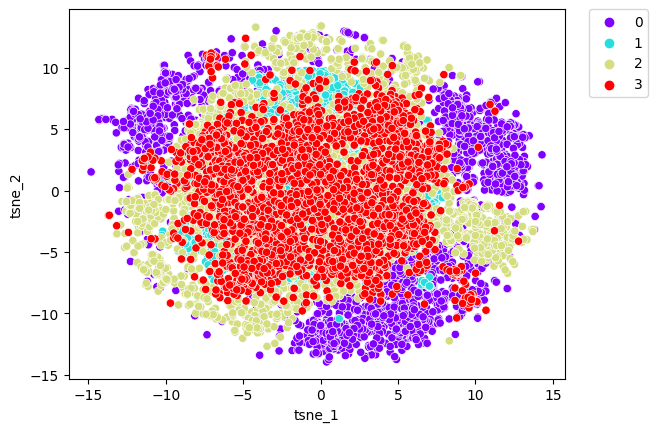
\includegraphics[width=1\linewidth]{Imagedata1/tsne1.png}
	\caption{ Διάγραμμα απεικονισμού κλάσεων }
	\label{f:g10}	
\end{figure}

\clearpage

\subsection{Spectral clustering with rbf}

Στο συγκεκριμένο αλγόριθμο, επιλέχθηκε να αλλάζει ο αριθμός των cluster και ορίστηκε ώς δείκτης ομοιότητας μεταξύ των σημείων των δεδομένων το rbf.
Τα αποτελέσματα φάνηκαν στις δύο μετρικές στον πίνακα \ref{tab:abc6}. Το καλύτερο αποτέλεσμα για την πρώτη μετρική δίνεται όταν oι cluster είναι 15 \ref{f:g12}, και για την δεύτερη όταν είναι 35 \ref{f:g13}.

\begin{table}[ht]
	\centering
	\caption{Μετρικές για διαφορετικές τιμές cluster}
	\begin{tabular}{l | l | l}
		Τιμή cluster & Silhouette score &  Homogeneity score\\
		\hline
		10 & 0.208 & 0.240\\
		15 & 0.227&0.243\\
		20 & 0.182 & 0.260\\
		\label{tab:abc6}
	\end{tabular}
\end{table}
\begin{figure}[ht]
	\centering
	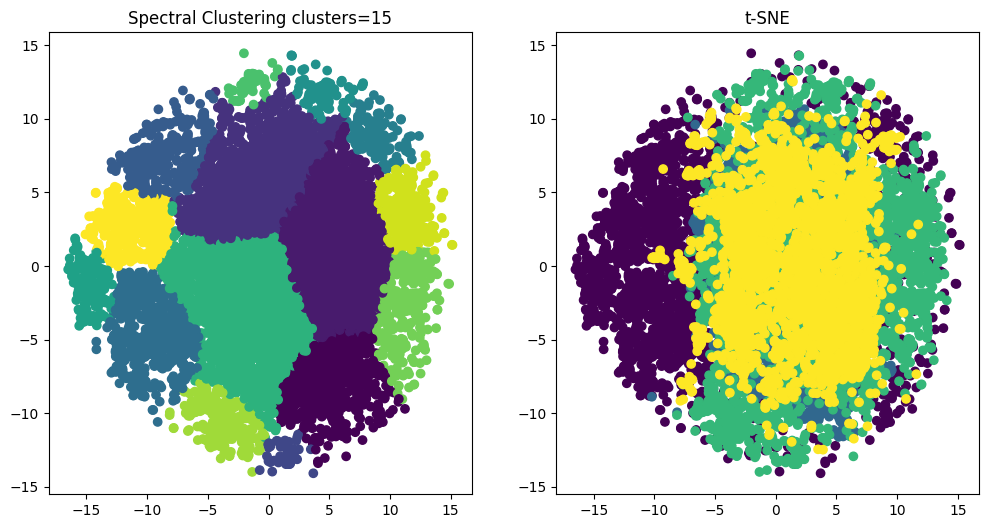
\includegraphics[width=1\linewidth]{Imagedata1/rbf_15tsne1.png}
	\caption{ Διαγράμματα σύγκρισεις απεικόνισης κλάσεων }
	\label{f:g12}	
\end{figure}

\begin{figure}[ht]
	\centering
	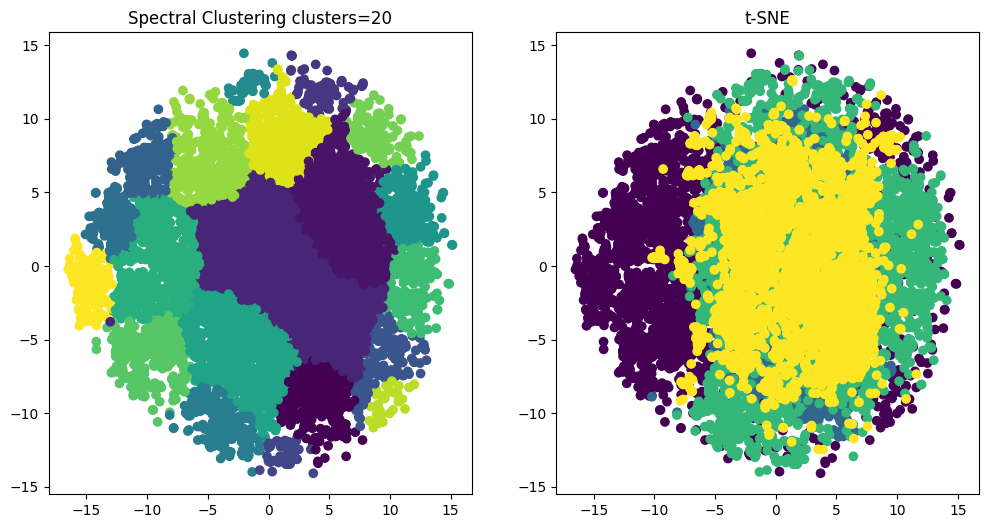
\includegraphics[width=1\linewidth]{Imagedata1/rbf_20tsne1.png}
	\caption{ Διαγράμματα σύγκρισεις απεικόνισης κλάσεων }
	\label{f:g13}	
\end{figure}
\clearpage

	\subsection{Spectral clustering with nearest neighbors}
	
	Στην συνέχεια αναπτύχθηκε ο ίδιος αλγόριθμος με διαφορετικό δείκτη ομοιότητας (affinity), ο οποίος είναι o nearest neighbors. Επιλέχθηκε να αλλάζει ο αριθμός των cluster και ο αριθμός των γειτόνων απο το 5 μέχρι το 40 με βήμα 5. Τα αποτελέσματα φάνηκαν στις δύο μετρικές στον πίνακα \ref{tab:abc7}. Το καλύτερο αποτέλεσμα για την πρώτη μετρική δίνεται όταν οι γείτονες και oι cluster είναι 30 \ref{f:g15}, και για την δεύτερη όταν είναι 35 \ref{f:g14}.
	
	\begin{table}[ht]
		\centering
		\caption{Μετρικές για διαφορετικές τιμές cluster/γειτόνων}
		\begin{tabular}{l | l | l}
			Τιμή cluster/γειτόνων & Silhouette score &  Homogeneity score\\
			\hline
			5 & -0.191 & 0.013\\
			10 & 0.319 & 0.179\\
			15 & 0.328&0.227\\
			20 & 0.321 & 0.266\\
			25 &0.336 & 0.290\\
			30 & 0.337 & 0.303\\
			35 & 0.333 & 0.306\\
		\end{tabular}

		\label{tab:abc7}
	\end{table}
	\begin{figure}[ht]
		\centering
		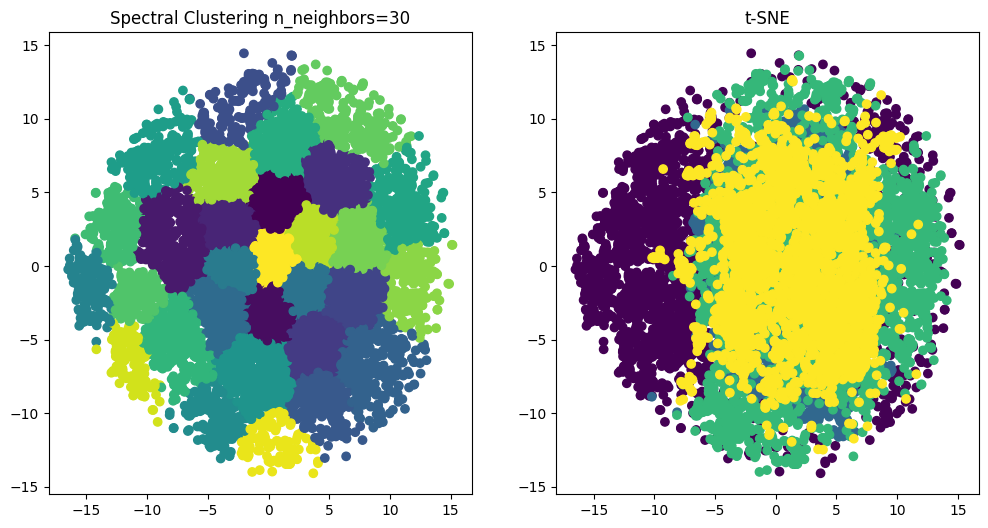
\includegraphics[width=1\linewidth]{Imagedata1/n_30tsne1.png}
		\caption{ Διαγράμματα σύγκρισεις απεικόνισης κλάσεων }
		\label{f:g15}	
	\end{figure}
	\begin{figure}[ht]
		\centering
		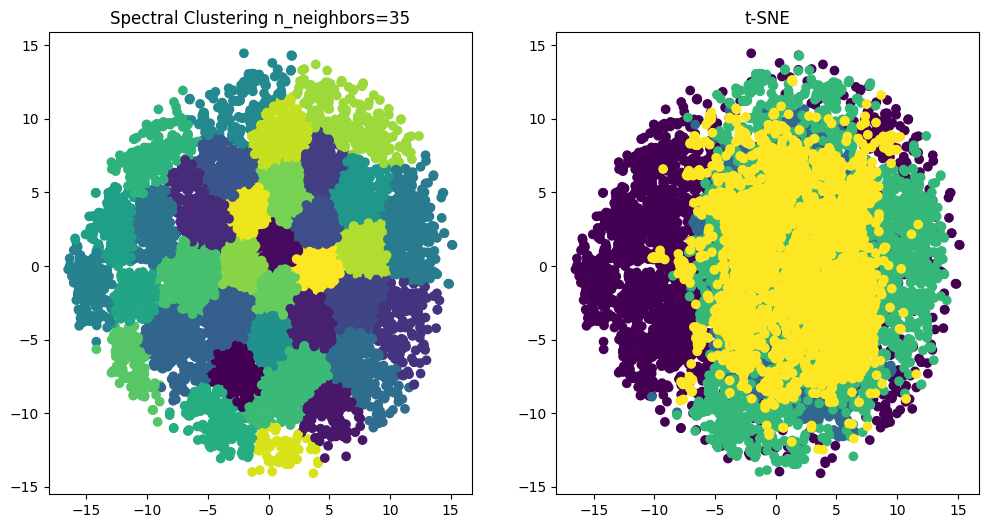
\includegraphics[width=1\linewidth]{Imagedata1/n_35tsne1.png}
		\caption{ Διαγράμματα σύγκρισεις απεικόνισης κλάσεων }
		\label{f:g14}	
	\end{figure}
	
	\subsection{Σύγκριση μεταξύ αλγορίθμων}
	Τα αποτελεσμάτα των μετρικών είναι παρόμοια στο spectral clustering με nearest neighbors και με rbf, και εξίσου χαμηλά.
	\clearpage
	
	\section{Isomap}
	Στην συνέχεια αναπτύχθηκε ο αλγόριθμος Isomap για την μέιωση των διαστάσεων σε δύο στο dataset. Ελέγχθηκαν διαφορετικές τιμές components στο isomap και όλες βγάλανε παρόμοια αποτελέσματα στις απεικονίσεις των διαγραμμάτων, για αυτό τον λόγο η διερέυνηση των αλγορίθμων Spectral clustering και kmeans έγινε με components = 2 στο Isomap.
	
	
	\subsection{Spectral clustering with rbf}
	
	Στο συγκεκριμένο αλγόριθμο, επιλέχθηκε να αλλάζει ο αριθμός των cluster και ορίστηκε ώς δείκτης ομοιότητας μεταξύ των σημείων των δεδομένων το rbf.
	Τα αποτελέσματα φάνηκαν στις δύο μετρικές στον πίνακα \ref{tab:abc8}. Το καλύτερο αποτέλεσμα για την πρώτη μετρική δίνεται όταν oι cluster είναι 10 \ref{f:g16}, και για την δεύτερη το αποτέσμα παραμένει το ίδιο.
	
	\begin{table}[ht]
		\centering
		\caption{Μετρικές για διαφορετικές τιμές cluster}
		\begin{tabular}{l | l | l}
			Τιμή cluster & Silhouette score &  Homogeneity score\\
			\hline
			10 & 0.103 & 0.012\\
			15 & 0.004&0.012\\
			20 & 0.013 & 0.012\\
			\label{tab:abc8}
		\end{tabular}
\end{table}		
		\begin{figure}[ht]
			\centering
			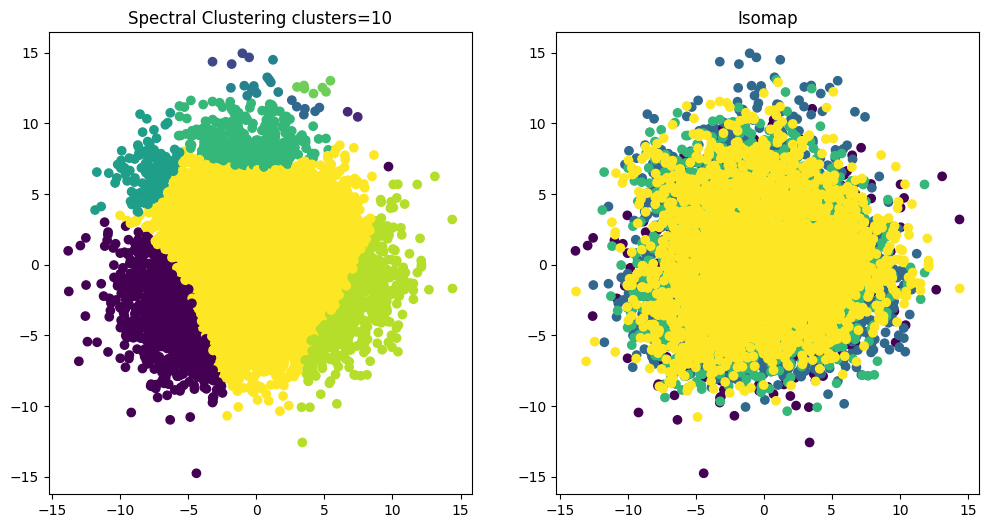
\includegraphics[width=1\linewidth]{Imagedata1/rbf_10isomap1.png}
			\caption{ Διαγράμματα σύγκρισεις απεικόνισης κλάσεων }
			\label{f:g16}	
		\end{figure}
		
		
		\subsection{Spectral clustering with nearest neighbors}
		
		Στην συνέχεια αναπτύχθηκε ο ίδιος αλγόριθμος με διαφορετικό δείκτη ομοιότητας (affinity), ο οποίος είναι o nearest neighbors. Επιλέχθηκε να αλλάζει ο αριθμός των cluster και ο αριθμός των γειτόνων απο το 5 μέχρι το 40 με βήμα 5. Τα αποτελέσματα φάνηκαν στις δύο μετρικές στον πίνακα \ref{tab:abc5}. Το καλύτερο αποτέλεσμα και για τη 1η μετρική δίνεται όταν ο αριθμός των cluster και των γειτόνων είναι 30 \ref{f:g17} και για την 2η όταν είναι 35 \ref{f:g18}
		
		\begin{table}[ht]
			\centering
			\caption{Μετρικές για διαφορετικές τιμές cluster/γειτόνων}
			\begin{tabular}{l | l | l}
				Τιμή cluster/γειτόνων & Silhouette score &  Homogeneity score\\
				\hline
				5 & -0.036 & 0.003\\
				10 & 0.277 & 0.016\\
				15 & 0.301&0.020\\
				20 & 0.282 & 0.022\\
				25 &0.288 & 0.024\\
				30 & 0.289 & 0.025\\
				35 & 0.288 & 0.026\\
			\end{tabular}
			
			\label{tab:abc5}
		\end{table}
		\begin{figure}[ht]
			\centering
			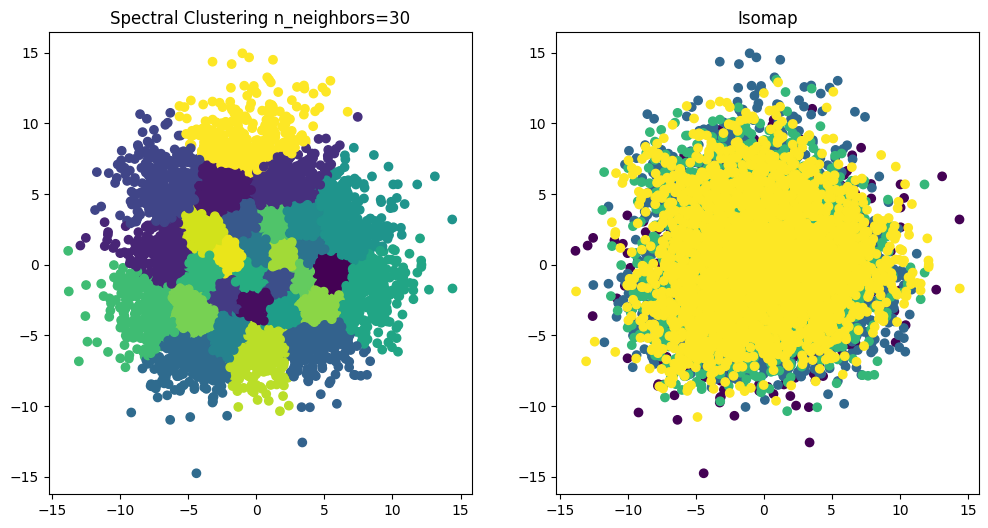
\includegraphics[width=1\linewidth]{Imagedata1/n_30isomap1.png}
			\caption{ Διαγράμματα σύγκρισεις απεικόνισης κλάσεων }
			\label{f:g17}	
		\end{figure}
		\begin{figure}[ht]
			\centering
			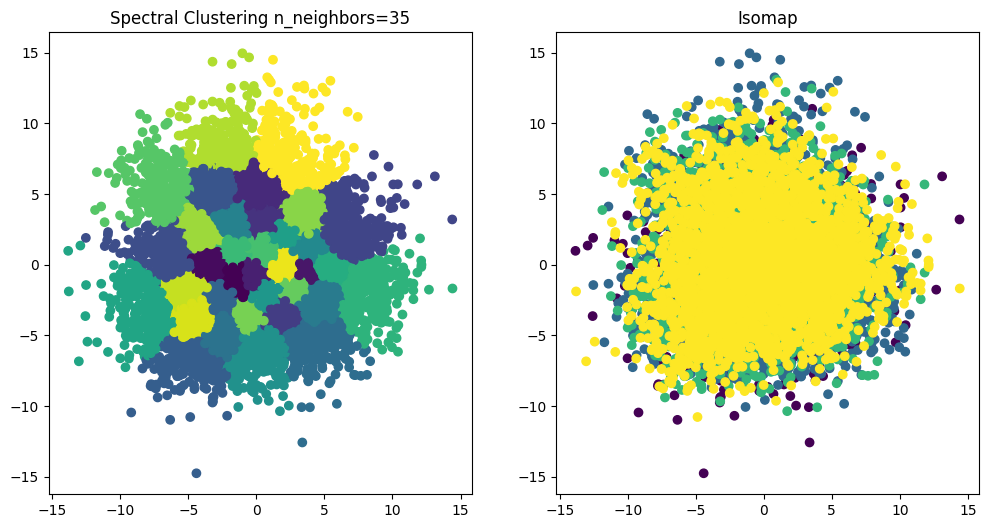
\includegraphics[width=1\linewidth]{Imagedata1/n_35isomap1.png}
			\caption{ Διαγράμματα σύγκρισεις απεικόνισης κλάσεων }
			\label{f:g18}	
		\end{figure}
		
\clearpage	
		
		\subsection{Σύγκριση μεταξύ αλγορίθμων}
		Τα αποτελεσμάτα των μετρικών είναι παρόμοια στο spectral clustering με nearest neighbors έχουν καλύτέρα αποτελέσματα απο αυτά τoυ rbf.
		
\section{Σύγκριση μεταξύ t-SNE και Isomap}

Το dataset στο οποίο αναπτύχθηκαν οι παραπάνω αλγόριθμοι δεν μας βοηθάει να βγάλουμε κάποια ερμηνεία για τα αποτελέσματα των δύο μετρικών. Αυτό συμβαίνει διότι τα σημεία των δεδομένω είναι πολύ κοντά μεταξύ τους και δεν μπορεί να γίνει καλός διαχωρισμός μετά απο μείωση διαστάσεων με τους αλγορίθμους t-SNE και Isomap. Οπότε παρόλο που τα αποτελέσματα είναι καλύτερα για τον πρώτο αλγόριθμο παραμένουν πάρα πολυ χαμηλά. Αυτο διακρίνεται σε μεγάλο βαθμό στα διαγράμματα απεικονισεις των κλάσεων.